\normalfont\normalsize
\chapter{Sparrow R}

Most of the nodes are build using AVR processor \cite{nodelist}, an 8-bit architecture. Few attempts have been made
using newer Arm Cortex-M3 32-bit architecture. The benefits of higher computing power are presented here
\cite{jurdak2011opal}, where a 4.6 throughput can be obtained compared to an 8-bit cpu over the
same wireless network. Unfortunately, the downside is higher power consumption that can create
difficulties for power supplies. Even though the same average power consumption can be obtained, due
to higher power peaks, the power supply energy will be depleted more quickly.

The current nodes, Sparrow V3.2 and SparrowV4, use an AVR 8-bit architecture and run at a speed of
16MHz. For our solar powered node, we wanted to use a newer, more powerful and lower power
microcontroller. Based on the previous requirements, we have chosen an Arm Cortex-M0+ 32-bit Atmel SamR21.


\section{\textit{Performance}}

We present bellow the main diferences between the two mcus, SAMR21 and ATMEGA128RFA1\cite{atmegafa}.

\begin{table} \centering
\begin{tabular}{llr}
\hline
Criteria    & Atmega128RFA1 & SamR21 \\
\hline
CPU Speed      & 16 MHz    & 48 MHz      \\
CPU architecture      & AVR 8bit    & Cortex M0+ 32bit      \\
CPU Power          & 4.1 mA       & 6.5 mA       \\
Flash           & 128 kB        & 256 kB        \\
Ram                 & 16 kB     & 32 kB         \\
Flash Endurance     &  50000    & 150000        \\
Rx Consumption       & 12.5 mA     & 11.8 mA     \\
Tx Consumption       & 14.5 mA @ 3.5mA     & 13.8 mA @ 4 dBm      \\
Receiver sensitivity & -100 dBm      & -101 dBm       \\
Tx Max Power & 3.5 dBm      & 4 dBm       \\
Package & QFN64      & QFN48 or QFN32      \\
\hline
\end{tabular}
\caption{Comparison between Atmega128RFA1 and SamR21}
\end{table}

\begin{table} \centering
\begin{tabular}{llllr}
\hline
Criteria    & Atmega128RFA1 & SamR21 & Total Advantage & Advantage per MHz \\
\hline
Integer Iterations      & 44890    & 403950   & 8.99 &  2.99 \\
Branch Iterations      & 27782    & 93552  &  3.36 &  1.12  \\
While(1) Iterations          & 191536     & 6693086    & 34.94  & 11.64  \\
\hline
\hline
\end{tabular}
\caption{Speed comparison}
\end{table}

\begin{table} \centering
\begin{tabular}{llr}
\hline
Criteria    & Atmega128RFA1 & SamR21 \\
\hline
Integer Iteration    &  274 nJ & 49 nJ \\
Branch Iteration      & 442 nJ & 208 nJ  \\
While(1) Iteration          & 64 nJ & 2.9 nJ \\
\hline
\hline
\end{tabular}
\caption{Energy efficiency comparison}
\end{table}

Being a 32-bit architecture, even though SAMR21 consumes 5.5mA
compared to 4.1mA of Atmega128RFA1, for simple 32-bit integer addition, SAMR21 consumes only 49nJ
per iteration while the 8-bit micro-controller consumes 274nJ, almost 5 times more. Considering
performance figures, SAMR21 was 9 times faster with 403950 iterations per second while
Atmega128RFA1 managed only 44890 iterations.

Testing the performance of branch predictor, revealed that the M0+ is only 12\% better than
the older 8-bit counterpart when running at the same speed, but thanks to the frequency difference,
it ends up being 3.36 times faster.


\begin{figure}[ht] \centering
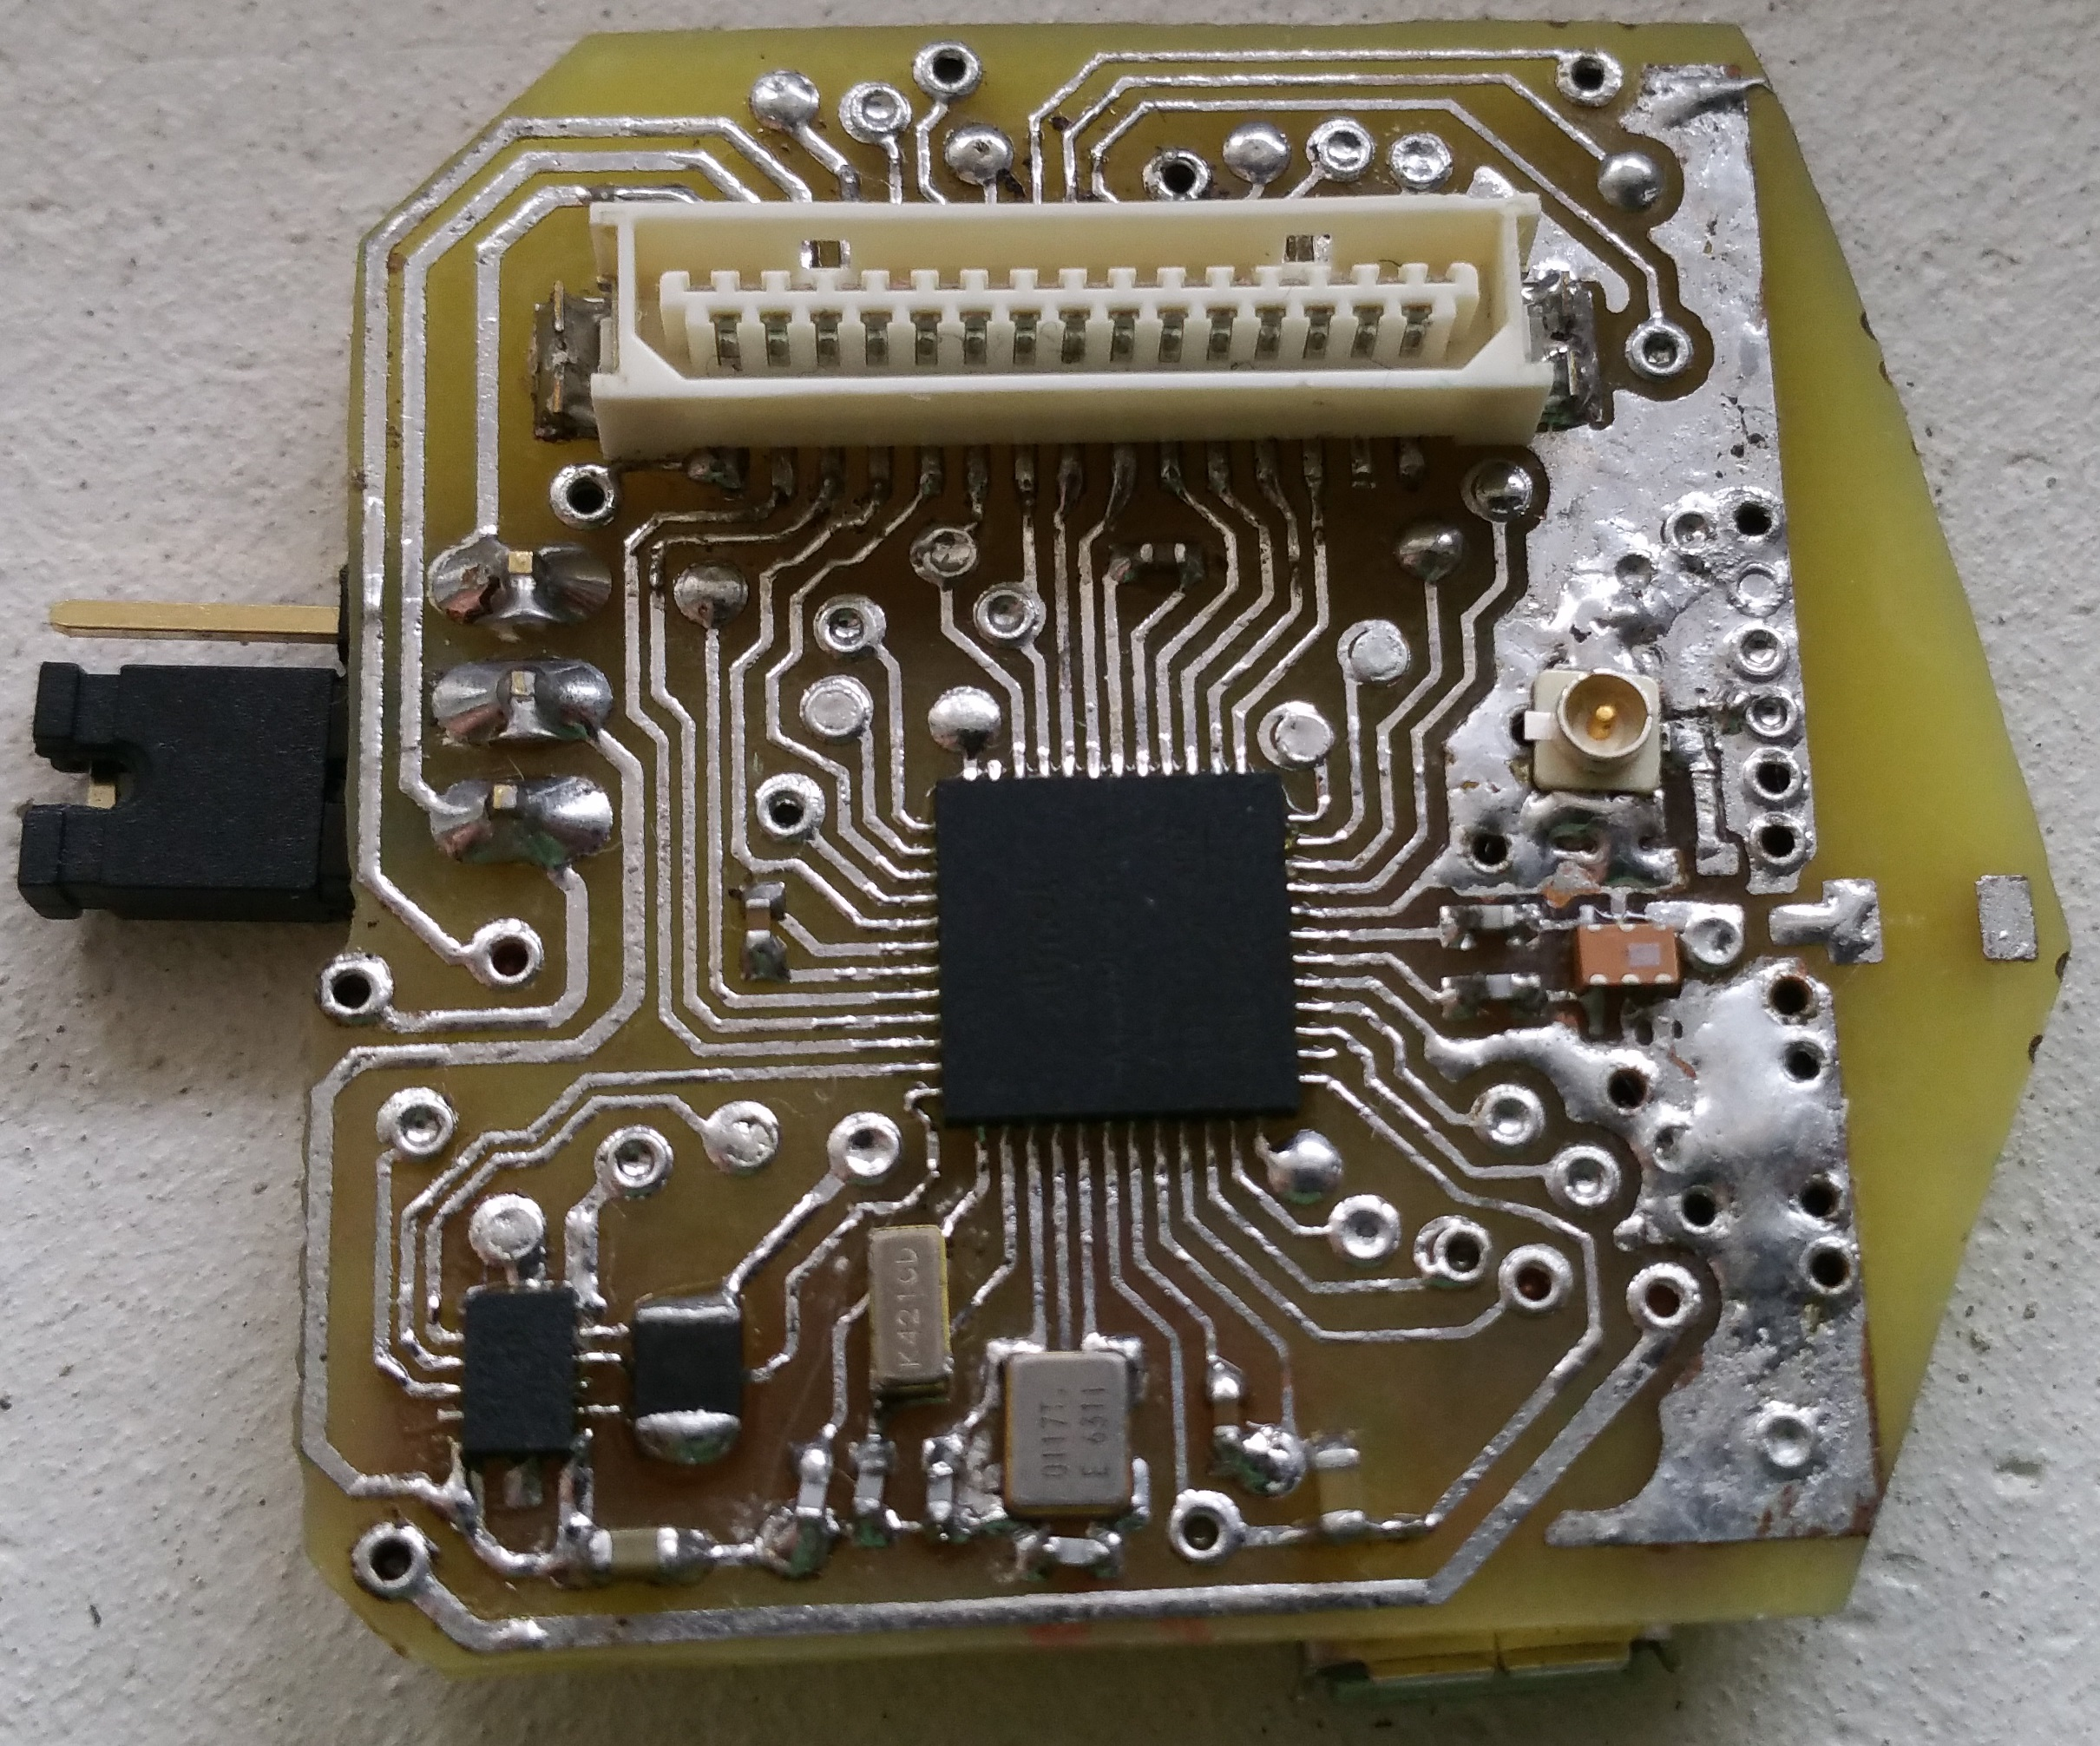
\includegraphics[width=0.85\textwidth]{img/sparrowrf.jpg}
\caption{Sparrow R node}
\end{figure}

The SAMR21 micro-controller is almost the same micro-controller as SAMD21 \cite{samd21}, which is used in Arduino
Zero boards. This allowed use to use exiting code, but unfortunately a not well
written one.

Even thought the Arduino software is well designed, it was not designed with low power approach
from the beginning. We will describe some of the problems encountered when trying to create the software stack.

The first problem noticed was that the Arduino Zero board had no sleep functionality implemented.
The ideal idle current consumption should have been less than 5uA, tested and measured using a
project created in Atmel Studio 7.0. The current consumption of the board was around 350uA. Further
tests revealed that the USB device was always initialized, which accounted for the extra 200
uA. The rest of 150uA came from a default initializations of the pins as input pins, but this only
lowered the current consumption to about 60uA. We kept searching for a cause, and discovered that
the clock generators are never disabled at start-up, which accounted for about 30uA.

So far we managed to decrease the idle current consumption for the platform from 350uA to about
30uA @ 3v2, but it is still far from ideal. Surprisingly, lowering the voltage from 3v2 to 1v8 lead
to  decrease in sleep current consumption down to 3.3uA. When examining the power trace using a digital oscilloscope, we found
that a very low frequency clock remains active, which at 3v2 has high spikes in power consumption.

Tough we did not reach the goal of 5uA, we still managed a respectable 30uA @ 3v2 and less than 4 uA @1v8.
Due to the time constrains and the need to use the nodes in order to implement and test new
features, we decided that for now this is acceptable, and for future revisions, we will come back
and find the extra clock source.

Even the run current consumption was not ideal, instead of achieving the promised 70uA/MHz @ 3v2,
or around 3.5mA @ 48MHz, the micro-controller consumed 8mA @ 48MHz. We managed to reduce the current consumption to 5.5mA @ 48MHz, due to
clock optimizations presented bellow.

The first change was to change the clock of the peripheral interfaces, instead of 48 MHz, we run them at 12 MHz.
Also if peripherals are not used, we completely disable them. Due to this, we ran into problems
related to SERCOM implementation, a generic module that handle USART, SPI and I2C. It was working
on Arduino Zero, because the CPU and the BUS were configured to run the same speed, but due to the
previous clock source modifications, the SERCOM did not set the correct speed. Also, there are 6
SERCOMs, and instead of enabling the clock for each one only when it is used, all of them were
enabled, which lead to extra power consumption during run time.

\begin{figure}[ht] \centering
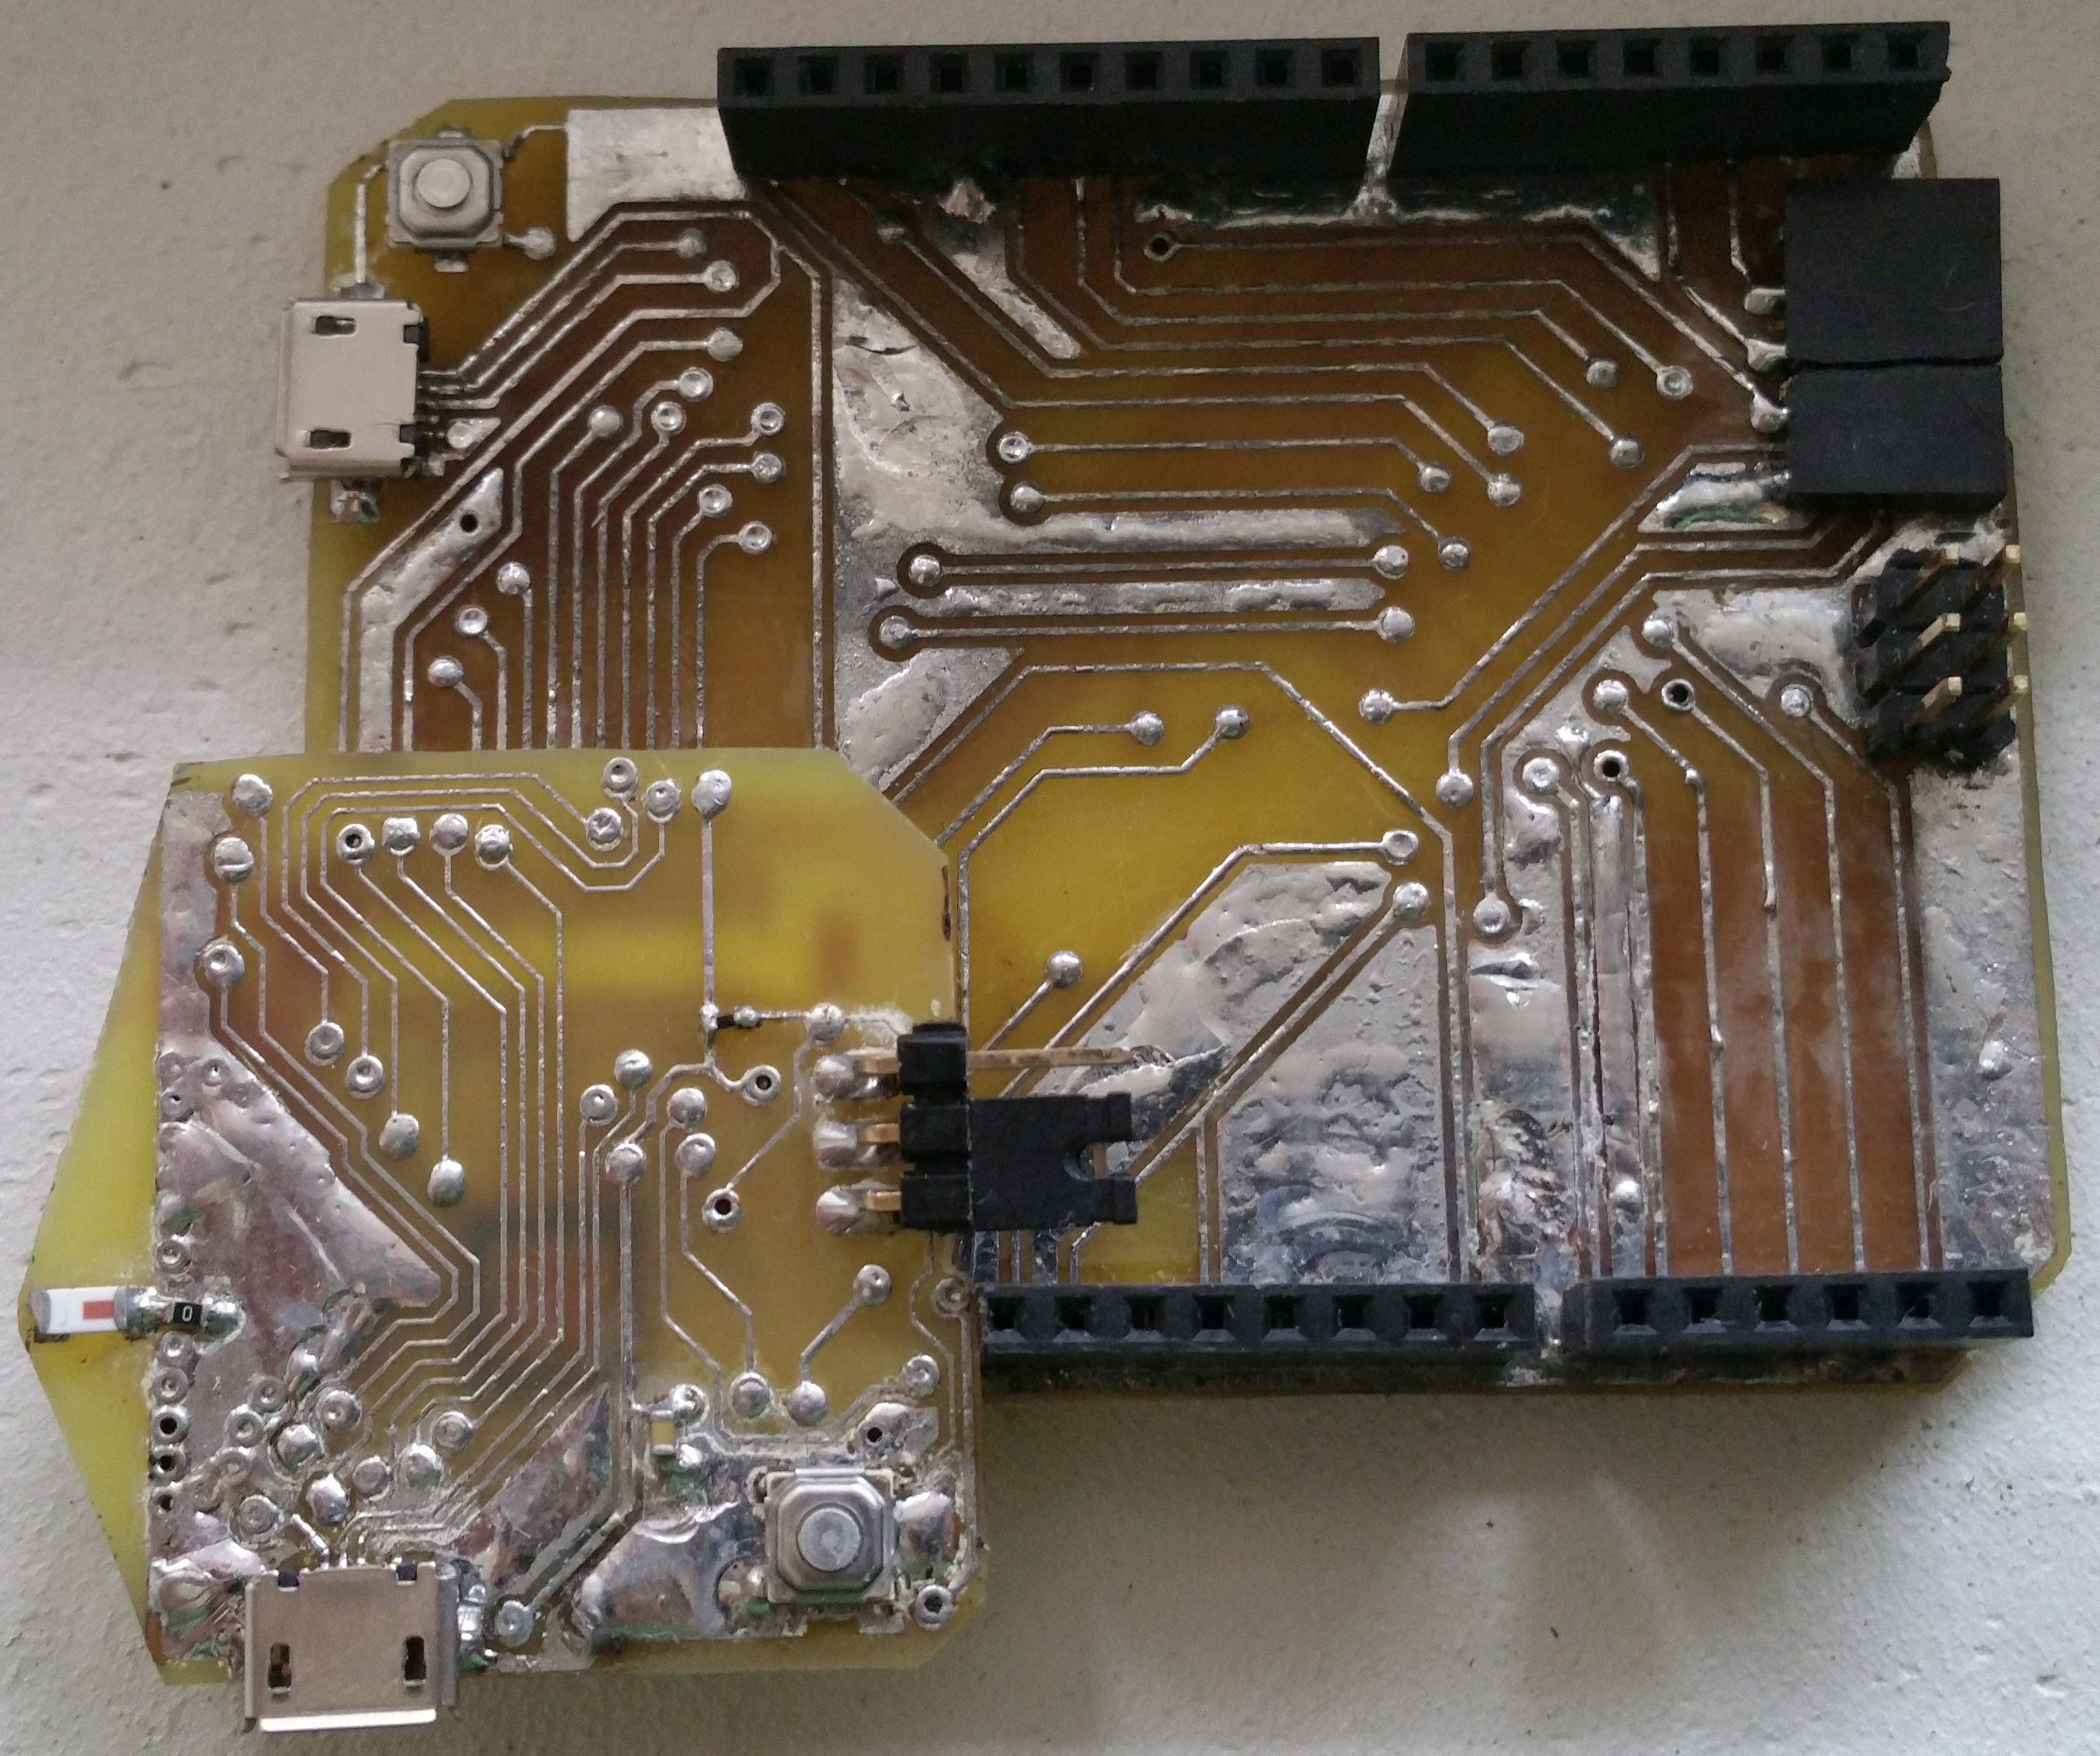
\includegraphics[width=0.85\textwidth]{img/base-with-sensor.jpg}
\caption{Sparrow R node mounted on Aduino compatible base}
\end{figure}

\section{\textit{Hardware}}
Because not all sensors are designed to run at 1v8 up to 3v3, we need to be able to dynamically
change the operating voltage of the node. We used TPS62742, a step-down switching DC/DC converter
with up to 90\% efficiency, voltage selectable output from 1v8 to 3v2 with 200mV step, 360nA
quiescent current and a special mcu controllable load output, with push-pull transistors. In
inactive state the load line is pulled to GND and when active is pulled to VCC. When active it
consumes 12uA, but compared to the controlled sensors, this should not be noticeable. Because this
allows to completely power down the sensors, the "stand-by" current consumption is 0uA and it also
eliminates the previous design problem of floating GND which allowed the sensors to "steal" power
from other pins and not be properly disabled.

The node can be connected to an extension daughter board which fully respects the Arduino pinout.
The advantage of this approach is that it allows to easily test and prototype new configurations in
order to be prepare the project in the shortest time possible. Also existing hardware designed for Arduino can work with this board,
which increased the number of compatible hardware. In total, 20 I/O pins are available, pins that
can be used for connecting sensors, either on the daughter board, or directly on a specialty
designed board.

A jumper can select whether the Node is powered from USB or from other 2v1+ voltage supply. Through
the same jumper a power measuring device can be used to monitor the total power consumption. In case the DC/DC converter is not
needed the node can use other power source.

\section{\textit{Software}}

We implemented new modules designed for low power like sleep, power management which can dynamical
change the running voltage between 1v8 to 3v2 when requested and enable or disable the LOAD power
line. This allows the user to select which voltage is better required for applications. For example,
some sensor must be powered at exactly 2v8 while others at 2v5 or lower. This module allows for
precise voltage selection with 200mV increments, use the sensor and then switch to the lowest
voltage in order to obtain the best power consumption possible.

The RF module is AT86RF233, integrated into the micro-controller. An Arduino library
\cite{rf233}
exists for the RF but in order to add new features, we integrated the module for the RF in the core
of the platform. This allowed us to let the user focus on what to do with the platform and not how to do
something with it. Furthermore, extra futures and bug fixes are easier to be implemented if the module is
integrated in the platform. For example, in case the RF is constantly running in receive mode for
more than 5 minutes, it is recommended to do Fine Tuning of the PLL clock in order to eliminate
possible clock skews. Feature wise, when the module automatically receives a packet, it saves it
locally together with RSSI and LQI, which can be later read and used buy the user. The internal
buffer is designed for 8 packets of 127KB of data, which amounts for 1 KB of ram. The buffer is
cyclic, so in case the buffer is not read, the oldest data is discarded and replaced by a new one.
This should not happen very often, because the buffer is large enough to handle all request, even
for high bandwidth transfers.

If the user has a need to save the data in case of power failure, the micro-controller has an
EEPROM like functionality which allows a 16KB region of flash to emulate EEPROM write endurance.
The flash contains pages of 64 bytes, and the EEPROM has an overhead of 4 bytes, which leaves 60
bytes for actual data. Also, for each page, another page must be reserved for further use.
The results is that out of 16KB used, the total amount of usable space left is $\frac{16*1024}{2}
* \frac{60}{64} = 7680 bytes$. This should be more than enough for normal use because the normal
endurance of 25k cycles of flash write and erase are increased to at least 150k, with typical
values reaching 600k cycles. If a new software is uploaded, the EEPROM zone is completely erased.

For timekeeping when sleeping, RTC functionality was implemented. Besides keeping the time, RTC
provides alarm interrupts for a special date, which can be configured to be triggered every
minute, every hour, every day, every month, every year, or only once. Together with another
peripheral named EventSys, periodic interrupts are provided and the interrupts interval can range
from once every second up to 128 times per second, with increments of power base 2.

Because the software and hardware are never perfect, a watchdog functionality is also implemented,
in order to avoid code lock-up or hardware failure due to extreme environment conditions.

The software can be installed as a new board for Arduino 1.6.x, latest iteration to date,
May 2016. It was tested using Windows 8.1, but it should be fully compatible with other operating systems as well.

The node has native USB which allows for code upload and also serial interface over CDC. Because no
extra components are needed, the same node can be configured to act as a gateway or
as a leaf.

\label{chap:results}


\section{Power Consumption}

Having a very low power consumption, a small solar panel together with a
small capacitor can be used as the main power supply.

For example, when a 1F capacitor is used with the voltage ranging from 3v3 to 2v1 the equivalent battery capacity would be

$$ \frac{F * (Vi - Vf)}{t} = \frac{1F * (3.3V - 2.1V)}{3600s} = 0.333mAh$$

The node is equipped with a DC/DC converter that can bring substantial power savings, depending on
the voltage of the power supply. A LDO wastes a lot off energy as the delta between the
voltages increases, were as DC/DC works best when the delta increases, or putting it simple, if an
LDO ouputs 1v8 and a chip consumes 5mA, the input current is almost the same 5mA regardless of the
input voltage. So even though the chip consumes 9mW, the total power consumed is actually 25mW. If
in the same situation, a DC/DC with a 90\% efficiency is used, then the input current would be :
$$Iin = \frac{Iout * Vout}{Vin*Efficiency} = \frac{5mA * 1.8V*100}{5v*90}= 2mA$$


we can ignore the quiescent current because it is very small, around 360nA. The total power
consumption in this case is 10mW for an output power of 9mW compared with the LDO which consumes
25mW in order to output just 9mW, a 250\% difference between them.

In a real world situation, when a battery or a capacitor is used, the difference between them is
smaller. We will present two cases, in order to better understand the influence of higher
voltage supply.

The minimum voltage will be 2v1 for DC/DC and 1v9 for LDO. The current consumption of the chip is
5.5mA, and a capacitor of 1F.

Case 1: Capacitor charged to 3v3.

$$T_{LDO} = \frac{C * (V_i - V_f)}{I}=\frac{1F * (3.3V - 2.1V)}{5.5mA} = 218.2s $$

$$E_i = \frac{C*V_i^2}{2} = \frac{1f*(3.3V)^2}{2} =5.445J$$
$$E_f = \frac{C*V_f^2}{2} = \frac{1f*(2.1V)^2}{2} =2.205J$$
$$E = E_i - E_f = 3.24J$$
$$P = V*I*E_{fficiency }= \frac{1.8V * 5.5mA * 90}{100} = 11mW$$
$$T_{DC} = \frac{E}{P} = \frac{3.24J}{11mW} =294.54s $$

$$Advantage = \frac{T_{DC} - T_{LDO}}{T_{LDO}} = \frac{294.54s - 218.2s}{218.2s} =  35\%$$

Case 2: Capacitor charged to 5v.

$$T_{LDO} = \frac{C * (V_i - V_f)}{I}=\frac{1F * (5V - 2.1V)}{5.5mA} = 527.27s $$

$$E_i = \frac{C*V_i^2}{2} = \frac{1f*(5V)^2}{2} =12.5J$$
$$E = E_i - E_f = 10.295J$$
$$T_{DC} = \frac{E}{P} = \frac{3.24J}{11mW} =935.91s $$

$$Advantage = \frac{T_{DC} - T_{LDO}}{T_{LDO}} = \frac{935.91s - 527.27s}{527.27s} = 77.5\%$$

At 3.3V the advantage is not that big, but at 5V we nearly double the battery life. Furthermore, using a LIPO
battery which will increase the advantage of the DC/DC.


